\documentclass{article}

\def\npart {II}
\def\nyear {2017}
\def\nterm {Lent}
\def\nlecturer{Prof. I. Grojnowski}
\def\ncourse{Algebraic Geometry}
\def\draft{Rough}
\ifx \nauthor\undefined
  \def\nauthor{Bhavik Mehta}
\else
\fi

\author{Based on lectures by \nlecturer \\\small Notes taken by \nauthor}
\date{\nterm\ \nyear}
\title{Part \npart\ -- \ncourse}

\usepackage[utf8]{inputenc}
\usepackage{amsmath}
\usepackage{amsthm}
\usepackage{amssymb}
\usepackage{enumerate}
\usepackage{mathtools}
\usepackage{graphicx}
\usepackage[dvipsnames]{xcolor}
\usepackage{tikz}
\usepackage{wrapfig}
\usepackage{centernot}
\usepackage{float}
\usepackage{braket}
\usepackage[hypcap=true]{caption}
\usepackage{enumitem}
\usepackage[colorlinks=true, linkcolor=mblue]{hyperref}
\usepackage[nameinlink,noabbrev]{cleveref}
\usepackage{nameref}
\usepackage[margin=1.5in]{geometry}

% Theorems
\theoremstyle{definition}
\newtheorem*{aim}{Aim}
\newtheorem*{axiom}{Axiom}
\newtheorem*{claim}{Claim}
\newtheorem*{cor}{Corollary}
\newtheorem*{conjecture}{Conjecture}
\newtheorem*{defi}{Definition}
\newtheorem*{eg}{Example}
\newtheorem*{ex}{Exercise}
\newtheorem*{fact}{Fact}
\newtheorem*{law}{Law}
\newtheorem*{lemma}{Lemma}
\newtheorem*{notation}{Notation}
\newtheorem*{prop}{Proposition}
\newtheorem*{question}{Question}
\newtheorem*{rrule}{Rule}
\newtheorem*{thm}{Theorem}
\newtheorem*{assumption}{Assumption}

\newtheorem*{remark}{Remark}
\newtheorem*{warning}{Warning}
\newtheorem*{exercise}{Exercise}

% \newcommand{\nthmautorefname}{Theorem}

\newtheorem{nthm}{Theorem}[section]
\newtheorem{nlemma}[nthm]{Lemma}
\newtheorem{nprop}[nthm]{Proposition}
\newtheorem{ncor}[nthm]{Corollary}
\newtheorem{ndef}[nthm]{Definition}

% Special sets
\newcommand{\C}{\mathbb{C}}
\newcommand{\N}{\mathbb{N}}
\newcommand{\Q}{\mathbb{Q}}
\newcommand{\R}{\mathbb{R}}
\newcommand{\Z}{\mathbb{Z}}

\newcommand{\abs}[1]{\left\lvert #1\right\rvert}
\newcommand{\norm}[1]{\left\lVert #1\right\rVert}
\renewcommand{\vec}[1]{\boldsymbol{\mathbf{#1}}}

\let\Im\relax
\let\Re\relax

\DeclareMathOperator{\Im}{Im}
\DeclareMathOperator{\Re}{Re}
\DeclareMathOperator{\id}{id}

\definecolor{mblue}{rgb}{0., 0.05, 0.6}


% preamble
\usepackage{tikz}
\usepackage{stmaryrd}
\usepackage{tikz-cd}
\newcommand{\A}{\mathbb{A}}
\newcommand{\F}{\mathbb{F}}
\newcommand{\proj}{\mathbb{P}}
\DeclareMathOperator{\Mat}{Mat}
\DeclareMathOperator{\chara}{char}
\DeclareMathOperator{\Mor}{Mor}
\DeclareMathOperator{\Gal}{Gal}
\DeclareMathOperator{\Der}{Der}
%\setcounter{section}{-1}
% and here we go!

\begin{document}
\maketitle
\tableofcontents

\section*{Introduction}
Consider $E = \set{(x, y) \in \C^2 | y^2 = x^3 - x}$. Let's first draw this when $(x, y) \in \R^2$.
If $y \in \R$, $y^2 \geq 0$, so if $x \in \R$, $x^3 - x = x(x^2 - 1) \geq 0$ so $x \geq 1$ or $-1 \leq x \leq 0$.

% draw picture!

Now consider $(x, y) \in \C$. In general, this is tricky.
Here, define $p: E \to \C$ given by $(x, y) \mapsto x$ most of the time ($x \notin \{0, 1, -1\}$), $p^{-1}(x)$ is two points.
This doesn't help us visualise.

\begin{equation*}
    \Gamma = \set{(x, y) \in \C^2 | y \in \R, x \in [-1, 0] \cup [1, \infty)}
\end{equation*}
Claim: $E \setminus \Gamma$ is disconnected and has two pieces.
Proof: Exercise.

So, $E \setminus \Gamma$ is two copies of
% pic
glued together. To glue, turn one of the pieces over (this ruins the representation as a double cover, but is the right gluing).
Think of (the picture below) by adding a point at $\infty$, so it lives on the Riemann surface.

Take another copy, flip it over and glue back.
(this section is in the process of tidying)

\clearpage
% I
\section{Dictionary between algebra and geometry}
% 1.
\subsection{Basic notions}
\begin{defi}[Affine space\hypertarget{def:affineSpace}]
    \textbf{Affine $n$-space} is $\A^n = \A^n(k) \coloneqq k^n$ for $k$ a field.
\end{defi}
\begin{notation}\hypertarget{def:polys}
    Write $k[\A^n] = k[x_1, \dotsc, x_n]$ for the polynomials in $n$ variables.
\end{notation}
Any $f \in \hyperlink{def:polys}{k[\A^n]}$ defines a function $f: \A^n =k^n \to k$ given by $(\lambda_1, \dotsc, \lambda_n) \mapsto f(\lambda_1, \dotsc, \lambda_n)$ by evaluation.

Let $S \subseteq k[x_1, \dotsc, x_n]$ be any subset of polynomials.
\begin{defi}[Affine variety\hypertarget{def:Z}]
    \begin{equation*}
        Z(S) = \set{\lambda = (\lambda_1, \dotsc, \lambda_n) \in \hyperlink{def:affineSpace}{k^n} | f(\lambda_1, \dotsc, \lambda_n) = 0 \text{ for all } f \in S}
    \end{equation*}
    is called the \textbf{affine variety defined by} $S$, the simultaneous zeros of all functions in $S$.
    $Z(S)$ is called an affine subvariety of $\A^n$.
\end{defi}

\begin{eg}
    \leavevmode
    \begin{enumerate}[label=(\roman*)]
        \item $\hyperlink{def:affineSpace}{\A^n} = \hyperlink{def:Z}{Z}(0)$.
        \item On $\A^1$, $Z(x) = \{0\}$, $Z(x-7) = \{7\}$.  If $f(x) = (x - \lambda_1)\dotsc (x-\lambda_n)$, $Z(f(x)) = \{\lambda_1, \dotsc, \lambda_n\}$.
            Affine subvarieties of $\A^1$ are: $\A^1$ and finite subsets of $\A^1$.
        \item On $\A^2$, $E=Z(y^2-x^3+x)$ we (will) have sketched when $k=\C$ and $k=\R$ in the introduction.
        \item For $k=\R$, we have
            \begin{figure}[!h]
                \centering
                \begin{tikzpicture}[scale=0.7]
                    \begin{scope}
                        \node at (0, 3) {$Z(x, y) = \{(0, 0)\}$};
                        \fill (0, 0) circle (1pt);
                    \end{scope}
                    \begin{scope}[xshift=5cm]
                        \node at (0, 3) {$Z(xy)$};
                        \draw (0, 2) -- (0, -2);
                        \draw (2, 0) -- (-2, 0);
                    \end{scope}
                    \begin{scope}[xshift=10cm]
                        \node at (0, 3) {$Z(y)$};
                        \draw (2, 0) -- (-2, 0);
                    \end{scope}
                    \begin{scope}[xshift=15cm]
                        \node at (0, 3) {$Z(y(y-1), x(y-1))$};
                        \fill (0, 0) circle (1pt);
                        \draw (2, 0.8) -- (-2, 0.8);
                    \end{scope}
                \end{tikzpicture}
            \end{figure}
            % diagrams of Z(x,y), Z(xy), Z(y) and Z(y(y-1),x(y-1))
    \end{enumerate}
\end{eg}

\begin{remark}
    If $f \in \hyperlink{def:polys}{k[\A^n]}$ then $\hyperlink{def:Z}{Z(f)}$ is called a \textbf{hypersurface}.
\end{remark}

Observe that if $J$ is the ideal generated by $S$
\begin{equation*}
    J = \Set{\sum a_i f_i | a_i \in k[x_1, \dotsc, x_n], f_i \in S}
\end{equation*}
then $\hyperlink{def:Z}{Z(J)} = Z(S)$.  Hence,
\begin{thm}
    If \hyperlink{def:Z}{$Z(S)$} is an affine subvariety of \hyperlink{def:affineSpace}{$\A^n$}, there is a finite set $f_1, \dotsc, f_r$ of polynomials with $Z(S) = Z(f_1, \dotsc, f_r)$.
\end{thm}

\begin{proof}
    $J = \langle f_1, \dotsc, f_r \rangle$ for some $f_1, \dotsc, f_r$ by Hilbert basis theorem.
\end{proof}

\begin{lemma}
    \leavevmode
    \begin{enumerate}[label=(\roman*)]
        \item if $I \subseteq J$, $\hyperlink{def:Z}{Z(J)} \subseteq Z(I)$
        \item $Z(0) = \hyperlink{def:affineSpace}{\A^n}$, $Z(\hyperlink{def:polys}{k[x_1, \dotsc, x_n]}) = \emptyset$.
        \item $Z\left(\bigcup J_i\right) = Z(\sum J_i) = \bigcap Z(J_i)$ for any possibly infinite family of ideals
        \item $Z(I \cap J) = Z(I) \cup Z(J)$ if $I, J$ ideals
    \end{enumerate}
\end{lemma}
\begin{proof}
    (i), (ii), (iii) are clear.

    (iv): $\supseteq$ holds by (i). Conversely, if $x \notin Z(I)$ then $\exists f_1 \in I$ such that $f_1(x) \neq 0$.
    So if $x \notin Z(J)$ also, $\exists f_2 \in J$ with $f_2(x) \neq 0$ also.
    Hence $f_1 f_2(x) = f_1(x) f_2(x) \neq 0$, so $x \notin Z(f_1 f_2)$. But $f_1 f_2 \in I \cap J$, as $I, J$ ideals so $x \notin Z(I \cap J)$.
\end{proof}

\begin{defi}[Zariski topology]
Looking at these results, $\hyperlink{def:Z}{Z(I)}$ form closed subsets of a topology on $\A^n$, called the \hypertarget{def:zariski}{\textbf{Zariski topology}}.
\end{defi}

\begin{defi}\hypertarget{def:I}
    If $Z \subset \A^n$ is any subset, set
    \begin{equation*}I(Z) \coloneqq \set{f \in \hyperlink{def:polys}{k[\A^n]} | f(p) = 0, \forall p \in Z}.\end{equation*}
\end{defi}
Observe that $\hyperlink{def:I}{I(Z)}$ is an ideal: if $g \in \hyperlink{def:polys}{k[\A^n]}$, $f(p) = 0$ then $(gf)(p) = 0$.
\begin{lemma}
    \leavevmode
    \begin{enumerate}[label=(\roman*)]
        \item $Z \subseteq Z' \implies \hyperlink{def:I}{I(Z')} \subseteq I(Z)$
        \item for any $Y \subseteq \hyperlink{def:affineSpace}{\A^n}$, $Y \subseteq \hyperlink{def:Z}{Z}(I(Y))$,
        \item if $V = Z(J)$ is a subvariety of $\A^n$, then $V = Z(I(V))$.
        \item if $J \lhd k[\A^n] = k[x_1, \dotsc, x_n]$ an ideal, then $J \subseteq I(Z(J))$.
    \end{enumerate}
\end{lemma}
\begin{proof}
    (i), (ii), (iv) are clear.
    For (iii), first show $\supseteq$. $I(V) = I(Z(J))\supseteq J$ by (iv) so $Z(I(V)) \subseteq Z(J)=V$ by (i). $\subseteq$ follows by (iv).
\end{proof}
Hence (ii) and (iii) show that $Z(I(Y))$ is the smallest affine subvariety of $\A^n$ containing $Y$, i.e.\ it is the closure of $Y$ in the \hyperlink{def:zariski}{Zariski topology}.

\begin{eg}
    Take $\Z \subseteq \C = \hyperlink{def:affineSpace}{\A^1}$, $k = \C$.
    If a polynomial in one variable vanishes at every integer, it is $0$, so $\hyperlink{def:I}{I(\Z)} = 0$ and hence the closure of $\Z$ in the \hyperlink{def:zariski}{Zariski topology} is $\C$.
\end{eg}

Note if $k = \C$, $f \in \hyperlink{def:polys}{\C[x_1, \dotsc, x_n]}$, then $f$ is continuous in the usual topology, so
\begin{equation*}
    \hyperlink{def:Z}{Z(J)} = \bigcap_{f \in J} Z(f) = \bigcap_{f \in J} f^{-1}(\{0\})
\end{equation*}
is a closed set in the usual topology, i.e. \hyperlink{def:zariski}{Zariski closed} $\Rightarrow$ closed in the usual topology.
So, the Zariski topology is coarser than the usual topology.

We now have maps
\begin{equation*}
    \begin{tikzcd}
    \begin{Bmatrix}
        \text{\hyperlink{def:zariski}{Zariski closed}} \\
        \text{subvarieties of } \hyperlink{def:affineSpace}{\A^n}
    \end{Bmatrix}
    \ar[r, bend right, hookrightarrow, "\hyperlink{def:I}{I}", start anchor=south, end anchor=south]&
    \begin{Bmatrix}
        \text{ideals in } \\
        \hyperlink{def:polys}{k[x_1, \dotsc, x_n]}
    \end{Bmatrix}
    \ar[l, bend right, two heads, "\hyperlink{def:Z}{Z}", start anchor=north, end anchor=north]
\end{tikzcd}
\end{equation*}
But this is not a bijection. For instance,
\begin{equation*}\hyperlink{def:Z}{Z(x)} = Z(x^2) = Z(x^3) = \dotsc = \{0\} \subseteq \hyperlink{def:affineSpace}{\A^1}.\end{equation*}
More generally,
$Z( f_1^{a_1}, \dotsc, f_r^{a_r}) = Z(f_1, f_2, \dotsc, f_r)$,
but it turns out this kind of thing is the only problem.
This is called Hilbert's `Nullstellensatz', and we will see it soon.
\begin{defi}[Reducible]
    An affine variety $Y$ is \textbf{reducible} if there are \hyperlink{def:Z}{affine varieties} $Y_1, Y_2$, $Y_i \neq Y$ with $Y = Y_1 \cup Y_2$, and \textbf{irreducible} otherwise. It is called \textbf{disconnected} if $Y_1 \cap Y_2 = \emptyset$.
\end{defi}

% UP TO HERE

% picsss
So $Z(xy) = Z(x) \cup Z(y)$, reducible.
$Z(y(y-1), x(y-1)) = Z(x,y) \cup Z(y-1)$ reducible and disconnected.
\begin{prop}
    Any affine variety is a finite union of irreducible affine varieties.
\end{prop}
\begin{remark}
    This is very different from usual manifolds.
\end{remark}
\begin{proof}
    If not, $Y$ is not irreducible, so $Y = Y_1 \cup Y_1'$ and one of $Y_1, Y_1'$, (say $Y_1$) is not the finite union of irreducible affine varieties, so
    \begin{equation*}
        Y_1 = Y_2 \cup Y_2', \dotsc
    \end{equation*}
    and so we get an infinite chain of affine varities $Y \supsetneq Y_1 \supsetneq Y_2 \supsetneq \dotsb$.
    But each $Y_i = Z(I_i)$ for some ideal $I_l$. Let $W = \bigcap Y_l = Z(\sum I_i) = Z(I)$.
    $I = \sum I_i$ is an ideal. As the ideal $I$ is finitely generated $I = \langle f_1, \dotsc, f_r \rangle$ for some $f_i$.
    $f_i \in I_{a_i}$ for some $a_1, \dotsc, a_r$ so $I = I_{a_1} + \dotsb + I_{a_r}$, $W = Y_{i_1} \cap \dotsb \cap Y_{i_r}$ contradicting $Y_N \subsetneq Y_{a_1} \cap \dotsb \cap Y_{a_r}$ if $N > r$.
\end{proof}
\begin{ex}
    If $Y$ is a subvariety of $\A^N$, then we can write $Y = Y_1 \cup \dotsb \cup Y_r$ with $Y_i$ irreducible, and $r$ minimal, uniquely up to reordering. Call the $Y_i$ the irreducible components of $Y$.
\end{ex}
\begin{prop}
    $Y$ is irreducible $\iff I(Y)$ is a prime ideal in $k[\A^n] = k[x_1, \dotsc, x_n]$.
\end{prop}
\begin{eg}
    \leavevmode
    \begin{enumerate}[label=(\roman*)]
        \item $(x y)$ is not a prime ideal.
        \item Exercise: Let $R$ be a UFD, $f \in R$, $f \neq 0$, $f$ irreducible $\iff (f)$ a prime ideal.
        \item Exercise: $k[x_1, \dotsc, x_n]$ is a UFD.
            Hence $Z(y^2 - x^3 + x)$ is irreducible, $Z(y-x^2)$ is irreducible.
    \end{enumerate}
\end{eg}
\begin{proof}
    If $Y = Y_1 \cup Y_2$ is reducible, $\exists p \in Y_1 \setminus Y_2$ so $\exists f \in I(Y_2)$ such that $f(p) \neq 0$ and similarly, $\exists q \in Y_2 \setminus Y_1$ so $\exists g \in I(Y_1)$ such that $g(q) \neq 0$.
    Then $fg \in I(Y_1) \cap I(Y_2) = I(Y)$. But $f \notin I(Y)$, $g \notin I(Y)$ so not prime.
    \begin{center}
        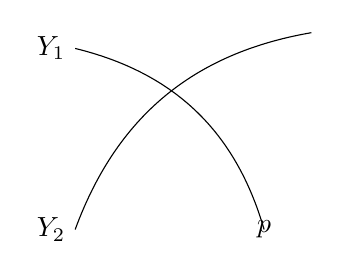
\begin{tikzpicture}
            \node [left] at (-1, 1.3) {$Y_1$};
            \node [left] at (-1, -1) {$Y_2$};
            \path (-1,1.3) edge [bend left=30] node[pos=1] {$p$} (1.4,-1) ;
            \draw (-1,-1) to[bend left=30] (2,1.5);
        \end{tikzpicture}
    \end{center}

    Conversely, if $I(Y)$ is not prime $\exists f_1 f_2 \in k[\A^n]$ such that $f_1, f_2 \notin I(Y)$ but $f_1 f_2 \in I(Y)$.
    Let $Y_i = Y \cap Z(f_i) = \set{p \in Y | f_i(p) = 0}$. $Y_1 \cup Y_2 = Y$, as $p \in Y \implies f_1 f_2 (p) = 0 \implies f_1(p) = 0$ or $f_2(p) = 0$.
    $Y_i \neq Y$ as $f_i \notin I(Y)$ (i.e. $\exists p_l \in Y$ such that $f_i(p_i) \neq 0$ so $p_i \notin Y_i$).
\end{proof}
\begin{lemma}
    $X$ irreducible affine subvariety of $\A^n$, $\mathcal{U} \subseteq X$ open and non-empty $\implies \overline{\mathcal{U}} = X$.
\end{lemma}
\begin{proof}
    Let $Y = X - \mathcal{U}$, closed. Then $\overline{\mathcal{U}} \cup Y = X$, and $\mathcal{U} \neq \emptyset \implies Y \neq X$. But $X$ is irreducible, so $\overline{\mathcal{U}} = X$.
\end{proof}

Application: Cayley-Hamilton Theorem
$A \in \Mat_n(k)$, an $n \times n$ matrix, with
\begin{equation*}
    \chara_A(x) = \det(x I - A) \in k[x]
\end{equation*}
the characteristic polynomial.
This gives a function $\chara_A: \Mat_n(k) \to \Mat_n(k)$ $B \mapsto \chara_A(B)$.
Cayley-Hamilton theorem says that $\forall A \in \Mat_n(k)$, $\chara_A(A) = 0$. Notice this is an equality of matrices, so it is $n^2$ equations.
\begin{proof}
    Let $X = \A^{n^2} = \Mat_n(k)$, affine space, hence irreducible algebraic variety.
    Consider $CH = \set{A \in \Mat_n(k) | \chara_A(A) = 0}$.
    Claim: this is a Zariski closed subvariety of $\A^{n^2}$, cut out by $n^2$ equations, $\chara_A(A)_y = 0$.
    We must check that these equations are polynomials in the matrix coefficients of $A$.

    %Lecture 3

    Consider $\chara_A(x) \in k[\A^{n^2 + 1}] = \det(xI - A)$, a polynomial in $x$ and in the matrix coefficients of $A$.
    \begin{equation*}
    \chara_{\begin{pmatrix}a & b//c&d\end{pmatrix}}(x) = \det
        \begin{pmatrix}
            x-a & -b \\ -c & x-d
        \end{pmatrix}
        =x^2  -(a+d) x + (ad - bc)
    \end{equation*}
    The $ij$th coefficient of $A^r$ is also a polynomial (of deg $r$) in the matrix coefficients of $A$, eg
    \begin{equation*}
        \begin{pmatrix}
            a & b \\ c & d
        \end{pmatrix}^2 =
        \begin{pmatrix}
            a^2 + bc & \dots \\
            \vdots & \ddots
        \end{pmatrix}
    \end{equation*}
    hence $\chara_A(A)_y=0$ is a poly in the matrix coefficients of $A$, proving the claim.

    Now, it is enough to prove the theorem when when $k = \overline{k}$, as $\Mat_n(k) \subseteq \Mat_n(\overline{k})$.
    Next, notice that $\chara_A(x) = \chara_{g A g^{-1}} (x)$, for $g \in \text{GL}_n$. and $\chara_A(g B g^{-1}) = g \chara_A(B) g^{-1}$ for $g \in \text{GL}_n$.
    Hence $\chara_A(A) = 0 \iff \chara_{g A g^{-1}}(g A g^{-1}) = 0$, so
    $A \in CH \iff g A g^{-1} \in CH$.
    Now, let $\mathcal{U} = \set{A \in \Mat_n(k) | A \text{ has distinct eigenvalues}}$. As $k = \overline{k}$, $A \in \mathcal{U} \implies \exists g \in \text{GL}_n$ with
    \begin{equation*}
        g A g^{-1} = \begin{pmatrix}
            \lambda_1 & 0 & \dots & 0 \\
            0 & \lambda_2 & \dots & 0 \\
            \vdots & \vdots & \ddots & \vdots \\
            0 & 0 & \dots & \lambda_n
        \end{pmatrix}
    \end{equation*}
    and it is clear that $g A g^{-1} \in CH$.
    As $k = \overline{k}$, $\#k$ is infinite, so $\mathcal{U}$ is non-empty so
    \begin{equation*}
        \emptyset \neq \mathcal{U} \subseteq CH \subseteq \A^{n^2} = X
    \end{equation*}
    hence if we show that $\mathcal{U}$ is Zariski open in $X$ then $\mathcal{U} = X$, as $X$ is irreducible. But $CH$ is closed, so $\mathcal{U} \subseteq CH$, so $CH=X$.

    Finally, we must show $\mathcal{U}$ is Zariski open.
    Observe $A \in \mathcal{U} \iff \chara_A(x) \in k[x]$ has distinct roots.
    Now recall from Galois theory, if $f(x)$ is a polynomial, $\exists$ poly $D(f)$ in the coefficients of the poly $f$ such that $f$ has distinct roots $\iff D(f) \neq 0$.

    So $A \in \mathcal{U} \iff D(\chara_A(x)) \neq 0$ is a polynomial in matrix coefficients of $A$.
\end{proof}

\subsection{Nullstellensatz}
Suppose $Y \subseteq \A^n$ is a subvariety,
let $I(Y) = \set{f \in k[x_1, \dotsc, x_n] | f(Y) = 0}$.
Recall we have maps
\begin{equation*}
    \begin{tikzcd}
        k[\A^n] \arrow[r] \arrow[rdd] & \{\text{functions from } k^n = \A^n \to k\} \arrow[dd] \\
                                     &\\
                         & \{\text{functions from } Y \to k\}
    \end{tikzcd}
\end{equation*}
where the composite is constructed by restricting a function from $\A^n \to k$ to $Y \to k$. Also note that the top map is injective if $\#k = \infty$.

\begin{defi}[Polynomial functions on subvariety]
    Let $k[Y] = k[x_1, \dotsc, x_n]/I(Y)$ by the \textbf{polynomial functions on $Y$}, also called \textbf{regular functions}.
\end{defi}
We just observed that $k[Y] \to \{\text{all functions from } Y \to k\}$ is injective if $\#k = \infty$.
We've seen $Y$ irreducible $\iff I(Y)$ is prime $\iff k[Y]$ is an integral domain.
Now let $p \in Y$. We have a map $k[Y] \to k$, given by $f \mapsto f(p)$.
This is an algebra homomorphism, so the kernel
\begin{equation*}
    m_p = \set{f \in k[Y] | f(p) = 0}
\end{equation*}
is an ideal. (The homomorphism is surjective as constants go to constants).
This is a maximal ideal, as $R/M$ a field $\iff M$ is a maximal ideal in $R$ and we have $k[Y]/m_p = k$.

A natural question to ask now is whether or not there are any other maximal ideals in $k[Y]$?
In particular, what are the possible surjetive algebra homomorphisms
\begin{equation*}
    k[x_1, \dotsc, x_n] \twoheadrightarrow L, \quad k \subseteq L, L \text{ field}.
\end{equation*}

For example, suppose $Y = Z(x^2+1)$ and $k=\R$. Then $k[Y] = \frac{\R[x]}{x^2 + 1}$ is not of the above form, since it is $\C$ instead of $\R$.

Claim: This is the only issue. If $k = \overline{k}$, there are no other algebra homomorphisms $k[Y] \to k$ other than evaluating at points $p \in Y$, and if $k \neq \overline{k}$ you just get for $L$ algebraic extensions of $k$, as in the above example.

\begin{thm}[Nullstellensatz, v1]
    Let $m \subseteq k[x_1, \dotsc, x_n]$ be a maximal ideal, and $A=k[x_1, \dotsc, x_n]/m$. Then $A$ is finite dimensional over $k$.
\end{thm}
\begin{remark}
    $A$ is finite dimensional over $k \iff$ every $a \in A$ is algebraic over $k$.
    (Proof: $\Rightarrow$ clear, as $1, a, a^2, \dotsc$ can't all be linearly independent over $k$. $\Leftarrow$ image of $x_1, \dotsc, x_n$ in $A$ each satisfy an algebraic relation over $k$ and they generate $A$).
\end{remark}
\begin{cor}
    If $k$ is algebraically closed, then $k \hookrightarrow A$ is an iso, ie $A \cong k$, that is, every maximal ideal is of the form $M= (x_1 - p_1, \dotsc, x_n - p_n)$ for $p \in k^n$.
\end{cor}
\begin{proof}
    $M$ a maximal ideal $\implies A$ a field, but if $k \subseteq \overline{k}$ that means $k = \overline{k}$ algebraic over $k$. Now let $a_i$ be the image of $x_i$ in $A$, and $M$ is as stated.
    So if $k = \overline{k}$, solutions of equations $I \longleftrightarrow$ max ideal $M \subseteq k[Y] \longleftrightarrow$ alg homomorphisms $k[Y] \to k$ and if $k \neq \overline{k}$, then they are `galois orbits of solutions over bigger fields'.
\end{proof}

% Lecture 4

We can interpret this in the case $k \neq \overline{k}$ as saying: to study solutions of algebraic equations over $K$, i.e. simultaneous zero of an ideal $I$, it is necessary to study their solutions over fields bigger than $k$, such as $\overline{k}$.
\begin{proof}
    When $k$ is uncountable: If the result is not true, $\exists t \in L\setminus k$ with $t$ transcendental over $k$. In particular, $k(t) \subseteq L$. SO $\frac{1}{t-\lambda} \in L, \forall \lambda \in k$.
    But $L$ has countable dimension over $k$ (let $V_d$ be the $k$-vector space which is the image of $\set{f \in k[x_1, \dotsc, x_n] | \deg f \leq d}$, $V_d$ is finite dimensional, $\bigcup V_d = L$).
    Now consider $\frac{1}{t-\lambda}, \dotsc, \frac{1}{t-\lambda_r}$ for $\lambda_1, \dotsc, \lambda_r \in k$ distinct. If these are linearly dependent over $k$, i.e. $\exists a_i \in k$ with $\sum \frac{a_i}{t - \lambda_i} = 0$, then clearing denominators gives a poly relation in $t$, contradicting $t$ is transcendental.
    So they are linearly independent, but there are uncountably many $\lambda \in k$, a contradiction.
\end{proof}

\begin{cor}
    If $k = \overline{k}$, take $I \leq k[x_1, \dotsc, x_n]$ an ideal.
    Then $Z(I) \neq \emptyset \iff I \neq k[x_1, \dotsc, x_n]$. More generally, $I \leq k[Y]$, $Z(I) \neq \emptyset \iff I \neq k[Y]$.
\end{cor}
Note if $k \neq \overline{k}$, this is obviously false.

\begin{proof}
    For $I \leq k[Y] = k[x_1, \dotsc, x_n]/I(Y)$, replace $I$ by its inverse image in $k[x_1, \dotsc, x_n]$ to see it suffices to prove the specific case instead of the general case.

    If $I \neq k[x_1, \dotsc, x_n]$, then $I \subseteq m \subsetneq k[x_1, \dotsc, x_n]$ for $m$ a maximal ideal. $I$ is contained in some maximal ideal. But Nullstellensatz gives $Z(m) = \{p\}$ for some $p \in k^n$.
    So $Z(I) \supseteq Z(m) = \{p\} \neq 0$.
\end{proof}

\begin{remark}
    This means, any ideal of equations which aren't all the equations have a simultaneous solutions.
    This is equivalent to the Nullstellensatz.
\end{remark}
\begin{defi}[Radical ideal]
    Take $R$ a ring, $J \lhd R$ an ideal.  The \textbf{radical} is
    \begin{equation*}
        \sqrt{J} \coloneqq \set{f \in R | \exists n \geq 1, f^n \in J } \supseteq J
    \end{equation*}
\end{defi}
\begin{lemma}
    $\sqrt{J}$ is an ideal.
\end{lemma}
\begin{proof}
    If $\gamma \in R$, $f \in \sqrt{J}$, then $(\gamma f)^n = \gamma^n f^n \in J$ if $f^n \in J$.
    If $f, g \in \sqrt{J}$ with $f^n \in J$, $g^m \in J$ for some $n, m$ then $(f+g)^{n+m} = \sum \binom{n+m}{i} f^i g^{n+m-i}$. Either $i \geq n$ so $f^i \in J$ or $n+m-i\geq m$ then $g^{n+m-i} \in J$, so $f+g \in J$.
\end{proof}

\begin{eg}
    \begin{enumerate}[label=(\arabic*)]
        \item $\sqrt{(x^n)} = (x)$ in $k[x]$.
        \item if $J$ is a prime ideal, $\sqrt{J} = J$.
        \item if $f \in k[x_1, \dotsc, x_n]$ is irreducible, then $(f)$ is prime as $k[x_1, \dotsc, x_n]$ is a UFD, so $\sqrt{(f)} = (f)$.
    \end{enumerate}
\end{eg}
Observe $Z(\sqrt{J}) = Z(J)$.
\begin{thm}[Nullstellensatz, v2]
    If $k = \overline{k}$, $I(Z(J)) = \sqrt{J}$.
\end{thm}
\begin{proof}
    Let $f \in I(Z(J))$, i.e. $f(p) = 0 \forall p \in Z(J)$. We must show that $\exists n$ such that $f^n \in J$.
    Consider $k[x_1, \dotsc, x_n, t]/tf-1 \coloneqq k[x_1, \dotsc, x_n, \frac{1}{f}]$.
    Let $i$ be the ideal of this, generated by the image of $J$.
    Claim: $Z(I) = \emptyset$. Proof: If not, let $p \in Z(I)$. As $J \subseteq I$, we have $p \in Z(J)$ and so $f(p) = 0$. But $p=(p_1, \dotsc, p_n, p_t)$ with $p_t \cdot f(p_1, \dotsc, p_n) = 1$, so $f(p) \neq 0$, contradiction.
    But now the corollary to Nullstellensatz version 1 gives $I=k[x_1, \dotsc, x_n, \frac{1}{f}]$. So, $1 \in I$. But $I$ is generated by $J$, so this says $1 = \sum_1^N \gamma_i/f^i$ for some $\lambda_i \in J$, $\gamma_N \neq 0$ for some $N$.
    Clear denominators and we get
    \begin{equation*}
        f^N = \sum \tilde{\gamma_i}, \tilde{\gamma_i} \in J, i.e. f^N \in J.
    \end{equation*}
\end{proof}
\begin{remark}
    This proof uses $k[x_1, \dotsc, x_n, t]/tf-1 \twoheadleftarrow k[\A^{n+1}]$. This is $k[Y]$, where $Y = Z(tf-1) \subseteq \A^{n+1}$ and $Z(tf-1) = \set{(p, t_0) | f(p) t_0 = 1}$.
    Clearly $Y \overset{\sim}{\rightarrow} \set{p \in \A^n | f(p) \neq 0} = \A^n \setminus Z(f)$.
\end{remark}
We will return to this, but first lets deduce some consequences of Nullstellensatz version 2.
\begin{cor}
    If $k = \overline{k}$, $Z(I) = Z(J) \iff I(Z(I)) = I(Z(J)) \iff \sqrt{I} = \sqrt{J}$.
    So we have a bijection
    % missing thing
\end{cor}
The intrinsic definition of affine varieties is a consequence (doesn't depend on the embedding of $X \hookrightarrow \A^n$).

\begin{defi}[Nilpotent]
    In a ring $R$, an element $y \in R$ is \textbf{nilpotent} if $y^n = 0$ for some $n > 0$.
\end{defi}
\begin{eg}
    In $k[x]/x^7$, $x$ is nilpotent.
\end{eg}
\begin{ex}
    Let $J \leq k[x_1, \dotsc, x_n]$ be an ideal, $R = k[x_1, \dotsc, x_n]/J$. Then $J = \sqrt{J} \iff R$ has no non-zero nilpotent elements.
\end{ex}
\begin{cor}
    Let $X \subseteq \A^n$ be a Zariski closed subvariety.
    Then $k[X]$ is a finitely generated $k$-algebra with no non-zero nilpotent elements.
    As it is finitely generated, there is $k[x_1, \dotsc, x_n] \overset{\alpha}{\twoheadrightarrow}k[X]$ a surjective algebra homomorphism and no non-zero nilpotents $\iff \ker \alpha$ is a radical ideal.
\end{cor}
\begin{defi}[Affine variety, v2]
    An affine variety over a field $k$ is a finitely generated $k$-algebra with no non-zero nilpotents.
\end{defi}
Observe:
\begin{enumerate}[label=(\roman*)]
    \item if $k = \overline{k}$, this coincides with our previous definition.
    \item if $k \neq \overline{k}$, we get new examples, now $\R[x,y]/x^2 + y^2 + 1$ is an affine algebraic variety over $\R$ even though $Z(x^2 + y^2 + 1) = \emptyset$.
        Note Nullstellensatz says $\R[x,y]/x^2 + y^2 + 1$ still has lots of maximal ideals but they correspond to $\Gal(\C/\R)$ orbits of complex solutions, i.e. complex conjugate pairs.
    \item this definition does not explicitly refer to a choice of embedding $X \hookrightarrow \A^n$ (the data of a choice of algebra generators for $k[X]$).
\end{enumerate}
What is missing? We still have to define what a map of algebraic varieties is.
\begin{defi}[Morphism]
    A \textbf{morphism} of algebraic varieties $X \to Y$ is a $k$-algebra homomorphism $f^*: k[Y] \to k[X]$. Write $\Mor(X, Y)$ for the set of morphisms, and write $f$ for the morphism associated to $f^*$.
\end{defi}
Let us unpack this definition.
Write
\begin{equation*}
    k[X] = k[x_1, \dotsc, x_n] / \langle s_1, \dotsc, s_l \rangle \qquad k[Y] = k[y_1, \dotsc, y_m] / \langle r_1, \dotsc, r_k \rangle
\end{equation*}
and write $\overline{y_1}, \dotsc, \overline{y_m}$ for the images of $y_i$ in $k[Y]$.
An algebra homomorphism $f^*: k[Y] \to k[X]$ takes $\overline{y_i} \mapsto f^*(\overline{y_i})$.
Choose a poly $\Phi_i = \Phi_i(x_1, \dotsc, x_n) \in k[x_1, \dotsc, x_n]$ which mod the ideal $\langle s_1, \dotsc, s_l \rangle$ equals $f^*(\overline{y_i})$.
This defines an algebra homomorphism
\begin{align*}
    k[y_1, \dotsc, y_m] &\longrightarrow k[x_1, \dotsc, x_n] \\
    y_l &\mapsto \Phi_i(x_1, \dotsc, x_n).
\end{align*}
Now the condition that this determines an algebra homomorphism $k[Y] \to k[X]$ is the condition that $r_i(\Phi_1, \dotsc \Phi_m) = 0$ in $k[X] \quad \forall i$ i.e. the ideal $\langle r_1, \dotsc, r_l\rangle$ get sent to zero in $k[X]$.
That is, $f^*$ is the data of polynomials $\Phi_1, \dotsc, \Phi_m$ in $k[x_1, \dotsc x_n]$ such that $r_i(\Phi_1, \dotsc \Phi_m) = 0$ (and the choice of such polynomials is well defined, up to adding any element of $\langle s_1, \dotsc, s_i\rangle$).
Moreover, $f^*$ determines a map of sets $X \to Y$, denoted $f:X \to Y$, $x \mapsto (\Phi_1(x), \dotsc, \Phi_m(x))$.
So, a morphism of algebraic varieties $f: X \to Y$ is, roughly speaking, a map of sets $X = (X_1, \dotsc, X_n) \in X \longrightarrow f(x) = (\Phi_1(x), \dotsc, \Phi_m(x)) \in Y$ (where $X \subseteq \A^n$ and $Y \subseteq \A^m$) given by polynomials $\Phi_1, \dotsc, \Phi_m \in k[\A^n]$. The condition that $(\Phi_1(x), \dotsc, \Phi_m(x)) \in Y$ is the condition $r_i(\Phi_1, \dotsc, \Phi_m) = 0$.
But, we gave this definition in a way which didn't require choosing $X \hookrightarrow \A^n$ etc.

\begin{defi}[Isomorphic]
    $X$ is \textbf{isomorphic} to $Y$ if $\exists \alpha^*: k[Y] \to k[X]$, $\beta^*: k[X] \to k[Y]$ such that $\alpha^* \beta^*$ and $\beta^* \alpha^*$ are identity.
\end{defi}
\begin{eg}
    \begin{enumerate}[label=(\roman*)]
        \item $t \mapsto (t^2, t^3)$ is a morphism $\A^1 \to \A^2$.
            More generally, $\Mor(\A^1, \A^n) = k$-algebra homomorphims $k[x_1, \dotsc, x_n] \to k[t]$ is just a tuple of polys $(\phi_1(t), \dotsc, \phi_n(t)) \in k[t]^n$.
        \item Take $\Mor(X, \A^1) \ni \varphi^*$, then $\varphi^* k[t] \to k[X]$ an algebra homomorphism. $k[t]$ is the free $k$-algebra on 1 generator $t$.
            That is, to specify an algebra homomorphism $k[t] \to R$ (for any ring $R$), it is enough to say where $t$ gets mapped to, and conversely any element of $R$ determines such a homomorphism.
            So $\Mor(X, \A^1) = k[X]$.
        \item $X = \A^1$, $Y = \set{(x, y) | x^2 = y^3} = Z(x^2 - y^3)$. Consider $t \mapsto (t^3, t^2)$. This is a morphism $(t^3)^2 = (t^2)^3$.
            Exercise: Is this an isomorphism? Is $Y \cong \A^1$?
        \item Take $\chara k \neq 2$. Is there a morphism $\A^1 \to \set{(x, y) | y^2 = x^3 - x}$ (which isn't a trival map).
            Do there exist polynomials $a = a(t), b=b(t) \in k[t]$, not both constant such that $b^2 = a^3 - a$.
    \end{enumerate}
\end{eg}

% Lecture 6

If $k = \overline{k}$, we can also reconstruct $f$ as follows
% points of x \longleftrightarrow max ideals m of k[X] <-> alg homs k[X] -> k
% now observe if $f^* : k[Y] \to k[X]$ and $x \in $X$, $ev_x: k[X] \to k$.
% get an alg homo $ev_x \cdot f^* : k[Y] \to k$, so the kernel is a maixmal ideal m_y$ for some y \in Y and f(x) = y
% ex: check f(x) = y

\begin{prop}
    Let $X$ be an affine algebraic variety, and $f \in k[X]$.  Then set \begin{equation*}Y = \set{(p, t) \in X \times \A^1 | t f(p) = 1}\end{equation*}.
    This is an affine algebraic variety, and the map $Y \hookrightarrow X$ with $(p, t) \mapsto p$ is a morphism of affine algebraic varieties.
\end{prop}
\begin{proof}
    It is $k[X] \to k[Y] \eqqcolon k[X][t]/tf-1$. Exercise: $k[Y]$ has no non-zero nilpotents.
\end{proof}
This means you should think of $Y \xrightarrow{\sim} X \setminus Z(f) \hookrightarrow X$.
That is, you should think of this as saying the Zariski open $X \setminus Z(f)$ is also an affine algebraic variety and the inclusion map $Y \hookrightarrow X$ is a morphism of algebraic varieties.

\begin{warning}
    Take $\set{(x, y) \in \A^2 | (x, y) \neq (0, 0)}$. This is Zariski open in $\A^2$ as $\{(0, 0)\}$ is a closed set. But, this is not an affine algebraic variety.
\end{warning}

\clearpage
\section{Projective space}
We will define it first as a set, then as an algebraic variety (but not an affine one).
Take $V$ a vector space over $k$, $\dim V = n+1$ for $n \geq 0$.
\begin{align*}
    \mathbb{P}V = \mathbb{P}^n &= \{\text{set of lines through } 0 \text{ in } V\} \\
                               &= (V \setminus \{0\}) /k^\times
\end{align*}
That is, if $v \in V$, $v \neq 0$ then $k v = \set{\lambda v | \lambda \in k}$ is a line through $0$, and conversely if $l \in \mathbb{P}V$ is a line, $l = kv$ for any $v \in l \setminus 0$.
Choose a basis $e_0, \dotsc, e_n$ of $V$, write $V \overset{\sim}{\leftarrow} k^{n+1}$, $\sum x_i e_i \mapsfrom (x_0, \dotsc, x_n)$. If $(x_0, \dotsc, x_n) \neq (0, \dotsc, 0)$, write $[x_0: \dotsc: x_n]$ for the corresponding point in $\mathbb{P}^n$ so $[\lambda x_0: \dotsc: \lambda x_n] = [x_0: \dotsc : x_n]$.
Claim: $\mathbb{P}^n = \A^n \amalg \mathbb{P}^{n-1}$.
Proof: Consider $[x_0 : \dotsc : x_n] \in \mathbb{P}^n$. Either $x_n = 0$ or $x_n \neq 0$.
If $x_n = 0$, $p = [x_0 : \dotsc : x_{n-1} : 0]$, and $p = p' = [x_0' : \dotsc : x_n']$ if and only if $x_n' =0$ and $\lambda(x_0, \dotsc, x_{n-1}) = (x_0', \dotsc, x_{n-1}')$ for some $\lambda \in k^\infty$, i.e. $p = p' \in \mathbb{P}^{n-1}$.
If $x_n \neq 0$, then we can rescale $(x_0, \dotsc, x_n) = x_n \cdot (\frac{x_0}{x_n}, \dotsc, \frac{x_{n-1}}{x_n}, 1)$, so get $\set{p \in \mathbb{P}^n | x_n \neq 0} \cong \A^n$. sending $[X_0 : \dotsc : X_n] \to (\frac{X_0}{X_n}, \dotsc, \frac{X_{n-1}}{X_n})$.
\begin{eg}
    $\mathbb{P}^1 = \A^1 \amalg \{\infty\}$ % picture
    Also, $\mathbb{P}^2 = \A^2 \amalg \mathbb{P}^1 = \A^2 \amalg \A^1 \amalg \A^0$.
    If $k = \F^q$, the number of points in $\mathbb{P}^n$ is $1 + q + \dotsc + q^n = \frac{q^{n+1}-1}{q-1}$.
\end{eg}
To phrase the above claim without coordinates, choose $H \leq V$ a vector subspace of codimension 1, and $w_0 \in V \setminus H$.
Then we have maps $\mathbb{P}H \hookrightarrow \mathbb{P} V \hookleftarrow H$ where the first map is $kv \mapsto kv$ and the second has $k(w_0 + h) \mapsfrom h$.
This gives $\mathbb{P}V \setminus \mathbb{P}H \overset{\sim}{\leftarrow} H$, in particular $\mathbb{P}V \setminus \mathbb{P}H \cong \A^n$.
So decomposition $\mathbb{P}V = \mathbb{P}H \amalg$ a space isomorphic to $\A^n$ depends only on the choice of a hyperplane $H$ but the isomorphism $\A^n \to \mathbb{P}V \setminus \mathbb{P}H$ depends on choice of $w_0 \in V \setminus H$.
Exercise: How does changing $w_0$ to $w_0'$ change the isomorphism?

% Lecture 7

% picture of n=1
% disjoint union of two copies of A1 (complex) surjects onto P1, and intersection is sphere missing both poles
% similar argument for P1 where A is real, (drawing nicely because of the action)

% GLn acts transitively on (n+1) hyperplanes when things intersect

% repeat for P2, taking A real again
So, $P^2 \twoheadleftarrow U_0 \amalg U_1 \amalg U_2$.
We have $U_i \cap U_j = \set{[x_0:\dotsm:x_n] | x_i \neq 0, x_j \neq 0} \cong \A^{n+1} \times (\A^1 \setminus \{0\})$.
The congruence here follows by embedding $U_i \cap U_j \hookrightarrow U_i$, and the image is points where $x_j/x_i \neq 0$.
In particular, we have $U_i \xrightarrow{\sim} \A^n$, with $x \mapsto (\frac{x_0}{x_i}, \dotsc, \frac{x_n}{x_i})$, where $1=x_i/x_i$ is omitted.
So, this lets us see projective space as covered by open sets (analogous to charts on a manifold).
% finitary data
% done in the handout apparently
\begin{defi}
    $X \subseteq \proj^n$ is Zariski closed if $X \cap U_i$ is Zariski closed in $U_i=\A^n$ for each $i=0, \dotsc, n$.
\end{defi}
Recall $E_0 = \set{(x, y) \in A^2 | y^2 = x^3 - x}$. Sit this inside $P^2 = [X:Y:Z]$ via $\A^2 \xrightarrow{\sim} U_2 = \{Z \neq 0\} \subseteq \proj^2$.
That is, $[X:Y:Z] \mapsto (x/z, y/z)$.
So, $x = \frac{X}{Z}$ and $y=\frac{Y}{Z}$. The equation $y^2 = x^3 - x$ becomes $Y^2/Z^2 = X^3 / Z^3 - X/Z$, and $Z \neq 0$ so the equation is $Y^2 Z = X^3 - XZ^2$ (for $Z \neq 0$).
Hence, $E_0 = \set{[X:Y:Z] | Y^2 Z = X^3 - X Z^2, Z \neq 0} \in \proj^2$.

% complement of three lines, so chart Y!=0 needs to miss out third line
On the chart $Z \neq 0$, we have the original equation $y^2 = x^3 - x$.
On $Y \neq 0$, take $x = \frac{X}{Y}$, $z = Z/Y$, i.e. set $Y=1$, get $z = x^3 - xz^2$ for $z \neq 0$.
For the chart $X \neq 0$, take $y = Y/X$, $z = Z/X$ get $y^2 z = 1 - z^2$ and $z \neq 0$.
So now take the closure of $E^0$ in $\proj^2$, which means ignore the condition $z \neq 0$. What, if any, extra points have we added?
On the chart $Y \neq 0$, if $Z = 0$ get $x^3 = 0$ the unique extra point $[0:1:0]$ % adding Z=0, Y!=0 back in gave one extra point
On the chart $X \neq 0$, if $Z=0$ get $1 = 0$, no solutions, so no extra points are added.
So, the closure of $E^0$ is $E_0 \amalg *$, just as we wanted.

More generally, if we have $I \leq k[x_1, \dotsc, x_n]$ an ideal, $Z = Z(I) \subseteq \A^n$, we can ask what the closure of $Z$ is in $\proj^n$ using $\A^n \to \proj^n$ given by $(x_1, \dotsc, x_n) \mapsto [1:x_1:\dotsm:x_n]$.

\begin{defi}\hypertarget{def:homPoly}
    $f \in k[x_0, \dotsc, x_n]$ is \textbf{homogeneous} of degree $d$ (for $d \geq 0$) if
    \begin{equation*}
        f = \sum a_{i_0, \dotsc, i_n} x_0^{i_0} \dotsm x_n^{i_n}
    \end{equation*}
\end{defi}
If $k$ is infinite, this is equivalent to $f(\lambda x) = \lambda^df(x)$ $\forall \lambda \in k^\times$.

As we saw in the example, given $f \in k[x_1, \dotsc, x_n]$ make $f$ homogeneous:
If $\deg f = d$, define $\tilde{f}(x_0, \dotsc, x_n) = x_0^d f(x_1/x_0, \dotsc, x_n/x_0)$ and then $\tilde{f}(1, x_1, \dotsc, x_n) = f(x_1, \dotsc, x_n)$ and $\tilde{f}(\lambda x_0, \dotsc, \lambda x_n) = \lambda^d \tilde{f}(x_0, \dotsc, x_n)$ $\forall \lambda \in k^\infty$ homogeneous of degree $d$.
For example, if $f = y^2 - x^3 + x$, $\tilde{f} = z^3 ((y/z)^2 - (x/z)^3 + (x/z))$ as in our example.
Define $\tilde{0} = 0$.
Observe
(i) if $f \neq 0$, then $x_0 \nmid \tilde{f}$, and conversely
(ii) if $x_0 \nmid g$, $g \in k[x_0, \dotsc, x_n]$ which is homogeneous of degree $d$, then $\tilde{g}(1, x_1, \dotsc, x_n) = g$.
\begin{defi}
    If $I \leq k[x_1, \dotsc, x_n]$ an ideal, define $\tilde{I} = \langle \tilde{f} | f \in I \rangle$ the ideal generated by the $\tilde{f}$.
\end{defi}
% important warning
\begin{warning}
    If $I = \langle f_1, \dotsc, f_r \rangle$ it need not be the case that $\tilde{I} = \langle \tilde{f_1}, \dotsc, \tilde{f_r}\rangle$
\end{warning}
\begin{eg}
    (i) Take $I = \langle x - y^2, y \rangle$. Note this is $\langle x, y \rangle$ and so the zero set is $\{0\}$. Now, $\langle \widetilde{x - y^2}, \tilde{y} \rangle = \langle xz - y^2, y \rangle = \langle xz, y\rangle$ but $\tilde{I} = \langle \tilde{x}, \tilde{y} \rangle = \langle x, y \rangle$.
    (ii)  Can you find an example of $I$ where $\tilde{I} \neq \langle \tilde{f_1}, \dotsc, \tilde{f_r} \rangle$ for any choice of $\langle f_1, \dotsc, f_r \rangle = I$ which has $r$ minimal.
\end{eg}

% Lecture 8
Notice that every polynomial $f\in k[x_0, \dotsc, x_n]$ can be written uniquely as $f = f_{(0)} + f_{(1)} + \dotsc$ where $f_{(i)}$ is homogeneous of degree $i$.
\begin{defi}
    An ideal $I$ is homogeneous if whenever $f \in I$, then $f_{(d)} \in I$ for all $d$.
\end{defi}
\begin{eg}
    $I = \langle x y + x^2, y^3 , x^2 \rangle$ is homogeneous (follows from following lemma) while $\langle x y + y^3 \rangle$ is not.
\end{eg}
\begin{lemma} \leavevmode
    \begin{enumerate}[label=(\roman*)]
        \item $I \leq k[x_0, \dotsc, x_n]$ is homogeneous $\iff I$ is generated by a finite set of \hyperlink{def:homPoly}{homogeneous} polynomials.
        \item Suppose $k$ is infinite. $\tilde{Z} = Z(I)$ is Zariski clsoed and invariant under multiplication by $k^\times$ i.e. $p \in \tilde{Z} \iff \lambda p \in \tilde{Z}, \quad \forall \lambda \in k^\times$ if and only if $I = I(\tilde{Z})$ is a homogeneous ideal.
    \end{enumerate}
\end{lemma}
\begin{proof}
    (i) $\Rightarrow$. $I$ is generated by some polynomials $g_1, \dotsc, g_n$. If $I$ is homogeneous, then the homogeneous parts $g_{i(j)}$ are in $I$, and they generate $I$. \\
    $\Leftarrow$. If $I = \langle g_1, \dotsc, g_n \rangle$, $g_i$ homogeneous of degree $d_i$.
    Let $h \in I$, so $h = \sum f_i g_i$.
    We have to show that $h = \sum h_{(d)}$ has each piece $h_{(d)} \in I$.
    But write $f_i = \sum f_{i,(k)}$, each $f_{i,(k)}$ homogeneous of degree $k$.
    Then regroup the sum $\sum f_{i, (k)} g_k$ as $h_{(d)} = \sum_{i : \deg(g_i) = d-k} f_{i, (k)} g_i \in I$.

    (ii) $\Leftarrow$. If $I = \langle g_1, \dotsc, g_n$ with $g_i$ homogeneous of degree $d$, then $g_i (\lambda p) = \lambda^{d_i} g_i(p) = 0$ if $g_i(p) = 0$, so $\tilde{Z}$ is invariant under $k^\times$. \\
    $\Rightarrow$. The group $k^\times$ acts on $k[x_0, \dotsc, x_n]$ as algebra automorphisms $\lambda * x_i = \lambda x_i$, with $(\lambda * f) (x_0, \dotsc, x_n) = f(\lambda x_0, \dotsc, \lambda x_n)$ and $Z(I)$ is $k^\times$ stable $\iff I$ is preserved by this action.
    That is, $f \in I \implies \lambda * f \in I$.
    So, let $f \in I$, $f = f_{(0)} + f_{(1)} + \dotsb$ with $\deg f_{(i)}  = i$. We must show $f_{(i)} \in I$.
    But $\lambda * f = f_{(0)} + \lambda f_{(1)} + \lambda^2 f_{(2)} + \dotsb$ so if we pick $\lambda_0 = 1$, $\lambda_1, \dotsc, \lambda_n \in k^\times$.
    \begin{align*}
        f = &\lambda_0 * f = f_{(0)} + f_{(1)} + f_{(2)} + \dotsb + f_{(n)} \\
            &\lambda_1 * f = f_{(0)} + \lambda_1 f_{(1)} + \lambda_1^2 f_{(2)} + \dotsb + \lambda_1^n f_{(n)} \\
        \vdots
            &\lambda_n * f = f_{(0)} + \lambda_n f_{(1)} + \lambda_n^2 f_{(2)} + \dotsb + \lambda_n^n f_{(n)} \\
    \end{align*}
    That is,
    \begin{equation*}
        \begin{pmatrix}
            1 & 1 & \dots & 1 \\
            1 & \lambda_1 & \dots & \lambda_1^n \\
            \vdots & \vdots & \ddots & \vdots \\
            1 & \lambda_n & \dots & \lambda_n^n \\
        \end{pmatrix}
        \begin{pmatrix}
            f_{(0)} \\f_{(1)} \\ \vdots \\f_{(n)}
        \end{pmatrix}
        =
        \begin{pmatrix}
            \lambda_0 \\ \lambda_1 \\ \vdots \\ \lambda_n
        \end{pmatrix}
        * f
    \end{equation*}
    So if we choose $\lambda_i \neq \lambda_j$ for all $i \neq j$ (possible as $\#k$ infinite), the determinant is
    \begin{equation*}
        \pm \prod_{i < j} (\lambda_i - \lambda_j) \neq 0
    \end{equation*}
    so we can invert the matrix and write $f_{(d)}$ as a linear combination of $\lambda_0 * f, \dotsc, \lambda_n * f$ all of which are in $I$.
    Hence $I$ is a homogeneous ideal.
\end{proof}
Recall $V = \A^{n+1}$, $H \leq \A^{n+1}$ a hyperplane, e.g.\ $H = \{x_0 = 0\}$, pick $p_0 \in V \setminus H$.
\begin{equation*}
    \A^n= \proj V \setminus \proj H \hookrightarrow \proj^n = \proj V
\end{equation*}
% (***) on the hook right arrow
$Z = Z(I) \subseteq \A^n \leadsto \tilde{I}$ a homogeneous ideal in $n+1$ variables, which generated the closure of $Z$ inside $\proj^n$.
In particular, the homogeneous ideal can be seen as defining a closed subvariety $\tilde{Z}$ of $\A^{n+1}$ such that $p \in \tilde{Z}$, then $\lambda p \in \tilde{Z} \; \forall \lambda \in k^\times$.
This corresponds to a closed subvariety of $\proj^n$ where $l \in $subvariety $\iff l = k p = \langle p \rangle$ for $p \in \tilde{Z}$, $p \neq 0$.
If $k = \overline{k}$, Nullstellensatz says this subvariety $\subseteq \proj^n$ is non-empty.
\begin{equation*}
    \iff \tilde{Z} \supseteq \{(0)\} \iff \text{ homogeneous ideal } I \lneq \langle x_0, \dotsc, x_n \rangle
\end{equation*}
i.e.\ Zariski closed subvarieties of $\proj^n \leftrightarrow$ homogeneous ideals in $x_0, \dotsc, x_n$ different from $\langle x_0, \dotsc, x_n \rangle$.
\begin{ex}
    Show that (***) defines a bijection
    % closed varieties of A^n <-> closed subvarities \overline{Z} of Pn such that no irreducible component of \overline{Z} is contains in \proj V \setminus \A^n = \proj H
    % Z \mapsto \overline{Z} = closure of I(Z) in \proj V
\end{ex}
\begin{defi}
    A projective variety is a closed subvariety of $\proj^n$, some $n$
\end{defi}
An affine variety is $k[X] = k[x_1, \dotsc, x_n]/I$, $I = \sqrt{I}$.
\begin{defi}
    A quasi-affine variety is an open subvariety of an affine variety
    A quasi-projective variety is an open subvariety of a projective variety.
\end{defi}
\begin{ex}
    If $\mathcal{U} \subseteq X$ an open subset of a variety $X$, $\exists$ structure of a variety on $\mathcal{U}$ makes the embedding a morphism of varieties.
\end{ex}

% Lecture 9
\section{Smooth points, dimension, Noether normalisation}
Let $X \subseteq \A^n$ be an affine variety, $p \in X$. Write $X = Z(I)$, $I = \langle f_1, \dotsc, f_r \rangle$.
We would like to think about the tangent space to $X$ at $p$, a vector space.
Our tentative definition is
\begin{align*}
    T_p X &= \set{v \in \A^n | \sum v_i \frac{\partial f_j}{\partial x_i}(p) = 0, j = 1,\dotsc, r} \\
    &= \set{v \in \A^n | \sum v_i \frac{\partial f}{\partial x_i}(p) = 0, \forall f \in I}
\end{align*}
For example, take $I = \langle y^2 - x^3 \rangle$.
% pic
Then
\begin{equation*}
    T_{(p_1, p_2)} X = \set{(v_1, v_2) | v_1 (-3p_1^2) + v_2 (2 p_2) = 0, -3p_1^2 v_1 + 2p_2 v_2 = 0}
\end{equation*}
So if $(p_1, p_2) \neq (0, 0)$ then $T_{(p_1, p_2)} X$ is a line, and if $(p_1, p_2) = (0, 0)$ then $T_{(p_1, p_2)} X = \A^2$.
\begin{remark}
    You can think of $T_p X$ as sitting at $p \in X$, by translating $v \mapsto v + p$.
    So,
    \begin{equation*}
        \simeq \set{v \in \A^n | \sum (v_i - p_i) \frac{\partial f}{\partial x_i} (p) = 0, \forall f \in I}
    \end{equation*}
    We can think of this as a linear approximation to the variety, $f(x) = f(p) + \sum (x_i - p_i) \frac{\partial f}{\partial x_i} + $ higher order terms.
\end{remark}
\begin{lemma}
    \begin{equation*}
        \set{p \in X | \dim T_p X \geq d}
    \end{equation*}
    is a Zariski closed subvariety of $X$, for all $d \geq 0$.
\end{lemma}
\begin{proof}
    \begin{equation*}
        T_p X = \ker
        \begin{bmatrix}
            \frac{\partial f_1}{\partial x_1} & \dots & \frac{\partial f_1}{\partial x_n} \\
            \vdots & \ddots & \vdots \\
            \frac{\partial f_r}{\partial x_1} & \dots & \frac{\partial f_r}{\partial x_n} \\
        \end{bmatrix}
    \end{equation*}
    and recall $\dim(\ker A) + r(A) = 0$.
    So, $\dim \ker \geq d \iff n - \text{rank} \geq d \iff rank \leq n - d$.
    But the rank of a matrix is greater than $a \iff$ exists some $a \times a$ submatrix with non-zero determinant.
    So, $\text{rank}(\frac{\partial f_j}{\partial x_i}) \leq d \iff \text{all } (n - d + 1) \times (n - d + 1)$ subminors have zero determinant which is a collection of polynomial equations.
    That is, $I \set{p \in X | \dim T_p X \geq d} = \langle f_1, \dotsc, f_r, \text{ determinants of all subminors} \rangle$.
\end{proof}
The problem with the definition from earlier was that it depends on an embedding, and we want a definition of $T_p X$ which doesn't depend on embedding $X \hookrightarrow \A^n$.
\begin{defi}\hypertarget{def:derivation}
    Take $A$ an algebra over $k$, and $\phi: A \to k$ a homomorphism. (For example, take $A = k[X]$, $\phi = \text{ev}_p: f \mapsto f(p)$.)
    A \textbf{derivation} `centered at $\phi$' is a $k$-linear map $D: A \to k$ such that
    \begin{equation*}
        D(fg) = D f \phi (g) + \phi(f) Dg \tag{Leibniz rule}
    \end{equation*}
    Write $\Der(A, \phi)$ for the set of such derivations, a vector space over $k$.
\end{defi}
\begin{eg}
    Take $A = k[x_1, \dotsc, x_n]$, $p \in \A^n$.
    If $(v_1, \dotsc, v_n) \in \A^n$, then $D(f) = \sum v_i \frac{\partial f}{\partial x_i} (p)$ is a \hyperlink{def:derivation}{derivation} centered at $\text{ev}_p$.
    Moreover, it is the unique derivation with $D(x_i) = v_i$.
\end{eg}
\begin{ex}
    Show it is unique.
\end{ex}
Conversely, given $D \in \Der(k[x_1, \dotsc, x_n], \text{ev}_p)$, get $v_i = D(x_i)$ so $\Der(k[x_1, \dotsc, x_n], \text{ev}_p) = T_p \A^n$.
More generally,
\begin{lemma}
    Let $A = \hyperlink{def:polys}{k[x_1, \dotsc, x_n]}/\langle f_1, \dotsc, f_r \rangle = k[X]$ and take $p \in X$.
    \begin{equation*}
        \Der(A, \text{ev}_p) = \set{D = \sum v_i \frac{\partial}{\partial x_i} |_p | D \langle f_1, \dotsc, f_r \rangle = 0 \text{ in } k[X]}
    \end{equation*}
\end{lemma}
\begin{proof}
    Can be seen as above.
    Alternatively, $\Der(k[X], \text{ev}_p)$ determines $\tilde{D} \in \Der(k[x_1, \dotsc, x_n], \text{ev}_p)$ and then the condition $\tilde{D}$ descends to a map $k[X] \to k$ is the condition $D\langle f_1, \dotsc, f_r \rangle = 0$.
\end{proof}
This gives us a better definition of tangent space:
\begin{defi}[Intrinsic definition of tangent space]
    \begin{equation*}
        T_p X = \Der(k[X], \text{ev}_p).
    \end{equation*}
\end{defi}
We can almost immediately conclude that this gives a definition for any algebraic variety.
\begin{ex}
    Let $V = X \setminus Z(f)$, $f \in k[X]$ be a Zariski open affine subvariety of $X$, i.e.\
    \begin{equation*}
        k[V] = k[X][\frac{1}{f}].
    \end{equation*}
    Show $T_p X \cong T_p X$ a canoncial isomorphism, i.e. that $\Der(k[X][\frac{1}{f}], \text{ev}_p) \xrightarrow{\sim} \Der(k[X], \text{ev}_p)$.
\end{ex}
So now $T_p X = T_p U$, for $U$ any Zariski open subvariety: the tangent space is Zariski local.
% pic

\begin{eg}
    Take $X = \proj^n$, $p = [p_0: p_1: \dotsb: p_n]$. If $p_0 \neq 0$, $p = [1: \frac{p_1}{p_0} : \dotsb : \frac{p_n}{p_0}] = \iota(\bar{p})$, the embedding of some $\bar{p} \in \A^n \hookrightarrow \proj^n$. THen
    \begin{equation*}
        T_p \proj^n = T_{\bar{p}} \A^n = \A^n
    \end{equation*}
\end{eg}
\begin{defi}
    Let $X$ be irreducible. Then the \textbf{dimension} of $X$:
    \begin{equation*}
        \dim X \coloneqq \min \set{\dim T_p X | p \in X}
    \end{equation*}
\end{defi}
\begin{eg}
    $\dim A^n = n = \dim \proj^n$, $\dim \set{(x, y) | y^2 = x^3} = 1$.
\end{eg}
If $X$ is not irreducible, the dimension is not such a great concept.
\begin{defi}
    If $X$ is arbitrary, $\dim X \coloneqq \max{\dim X_i | X_i \text{ a \hyperlink{def:component}{component} of } X}$.
\end{defi}
\begin{defi}
    If $X$ is irreducible, $p \in X$ is \textbf{smooth} if $\dim T_p X = \dim X$, and singular otherwise and we've shown singular points in $X$ form a Zariski closed subvariety, whose complement is non-empty. % (lemma from earlier in lecture)
\end{defi}
\begin{lemma}
    Let $f \in k[x_1, \dotsc, x_n]$ be prime. Then $\dim Z(f) = n-1$. Call this a `hypersurface'.
\end{lemma}
\begin{proof}
    $T_p Z(f)$ has dimension $n$ or $n-1$, and $T_p Z(f) = \A^n \iff \forall i \, \frac{\partial f}{\partial x_i} = 0$.
    So $T_p Z(f)$ has dimension $n$ for all $p \in Z(f) \implies \frac{\partial f}{\partial x_i} \in I(Z(f)) \quad \forall i=1, \dotsc, n$.
    But $I(Z(f)) = \sqrt{f}$, by Nullstellensatz, so $=(f)$ as $f$ is prime.
    So, $\frac{\partial f}{\partial x_i} = f . g$ for some $g$. But $\deg x_i \frac{\partial f}{\partial x_i} < \deg_{x_i} f \implies g = 0$.
    So $\dim Z(f) = 0 \implies \frac{\partial f}{\partial x_i} = 0 \quad \forall i$.
    There are now two cases,
    \begin{enumerate}[label=(\roman*)]
        \item if $\chara k = 0$, this implies $f = 0$.
        \item if $\chara k = p$, this implies $f \in k[x_1^p, \dotsc, x_n^p]$ as $\frac{\partial (x^p)}{\partial x} = p x^{p-1} = 0$.
    \end{enumerate}
    Claim: $\exists g \in k[x_1, \dotsc, x_n]$ such that $g(x)^p = f(x)$.
    Proof: If $f = \sum a_\lambda x^{\lambda p}$, $g = \sum a_\lambda^{1/p} x^\lambda$ (for $a_\lambda \in k$) which requires can take $p$th roots of things in $k$, which is allowed if $k = \bar{k}$.
    But this contradicts $f$ is prime!
\end{proof}
% Lecture 10
There are two other notions of dimension:
\begin{enumerate}[label=(\arabic*)]
    \item Krull dimension:
        \begin{equation*}
            \dim_{Kr} X = \max\set{r | \emptyset \neq Z_0 \lneq Z_0 \lneq Z_1 \lneq \dotsb \lneq Z_r = X}
        \end{equation*}
        where each $Z_i$ is an irreducible Zariski closed subvariety.

        For example, take $\A^1$. The only such chains are $\text{point} \lneq \A^1$, so $\dim_{Kr} \A^1 = 1$.
        We won't have time show show $\dim_{Kr} X = \dim X$.
    \item If $X$ is affine and irreducible, define $k(X)$ as the field of fractions of $k[X]$, which is non-zero as $k[X]$ is an integral domain.
        This is
        \begin{align*}
            k(X) &= \set{f/g | f, g \in k[X]} \\
                 &= \bigcup_{g \in k[X]} k[X \setminus Z(g)] \\
                 &= \bigcup_{g \in k[X]} k[X][\frac{1}{g}] \\
                 &= \bigcup_{U \subseteq X} \text{Zar. open, affine} k[U]
        \end{align*}
        called the function field of $X$.
        Observe that if $U \subseteq X$ is affine and open, then $k(U) = k(X)$.
        But this means that if $X$ is any irreducible variety, affine or not, can define $k(X) = k(U)$, for $U$ any affine open subset of $X$.

        Examples:
        \begin{enumerate}[label=(\roman*)]
            \item $k(\A^n) = k(x_1, \dotsc, x_n)$
            \item $k(\proj^n) = k(\frac{x_1}{x_0}, \dotsc, \frac{x_n}{x_0}) \simeq k(\frac{x_0}{x_n}, \dotsc, \frac{x_{n-1}}{x_n})$ since $\frac{x_i}{x_0} \cdot \frac{x_0}{x_n} = \frac{x_i}{x_n}$.
            \item if $E = \set{(x, y) | y^2 = x^3 - x}$, then $k(E) = k(x)[y]/y^2 = x^3 - x$
            \item $X = \set{(x, y) | y^2 = x^3}$, $k(X) = k(x)[y] / y^2 = x^3$
        \end{enumerate}

        Now we can define $\text{trdim} X =$ the transcendance dimension of extension $k \subseteq k(X)$.
        We need a small lemma to show trdim $k(x_1, \dotsc, x_n)/k = $ trdim $\A^n$ = n.
\end{enumerate}
\begin{thm}
    For any algebraic variety $X$ trdim $X = \dim X$.
\end{thm}
Proof strategy: We will reduce this to $\A^n$ where we know $\dim \A^n = n = \text{trdim} \A^n$ by looking for very special nice morphisms $X \to \A^n$.
To motivate this, consider the following special situation.
Suppose $k = \overline{k}$ and take a morphism $\varphi: X \to Y$ of affine varieties such that
\begin{enumerate}[label=(\arabic*)]
    \item $X, Y$ are irreducible
    \item \begin{equation*}
        k[X] = k[Y][t]/\langle f(t) \rangle
        \end{equation*}
        and $\varphi$ is the inclusion $k[Y] \hookrightarrow k[Y][t]/\langle f\rangle = k[X]$ where $f(t) \in k[Y][t]$,
        \begin{equation*}
            f(t) = a_0(y) + a_1(y)t + \dotsb + a_N(y) t^N = f(y, t) \quad \text{with } a_N \neq 0
        \end{equation*}
    \item $f$ is a separable polynomial, when regarded as an element of $k(Y)[t]$, i.e.\
        \begin{equation*}
            F(t) = \frac{f(t)}{a_N(y)} = t^N + \frac{a_{N-1}}{a_N} t^{N-1} + \dotsb + \frac{a_0}{a_N}
        \end{equation*}
        is such that $F(t), F'(t)$ have no common roots i.e.\ $\varphi X \to Y$ comes from a separable algebraic extension of function fields $k(X) \supseteq k(Y)$.
\end{enumerate}
In this situation, we have a lemma
\begin{lemma}
    \leavevmode
    \begin{enumerate}[label=(\alph*)]
        \item $\varphi(X)$ contains an open (hence dense!) subset of $Y$
        \item exists an open non-empty subset $V \subseteq Y$ such that $\varphi^{-1}(V)$ is finite, $\# \varphi^{-1}(v) \leq N, \; \forall v \in V$.
    \end{enumerate}
\end{lemma}
\begin{proof}
    (b). $X = \set{(y_0, t_0) \in Y \times \A^1 | f(y_0, t_0) = 0}$ and the morphism $X \to Y$ sends $(y_0, t_0) \mapsto y_0$.
    Now for fixed $y_0 \in Y \setminus Z(a_N)$, $f(y_0, t)$ is a polynomial in $k[t]$ of degree $N$ so has at most $N$ roots.
    (a). Let $U = \set{y \in Y | a_N(y) \neq 0} = Y \setminus Z(a_N)$ is Zariski open.
\end{proof}
\begin{ex}
    If $f: X \to Y$ is a morphism of affine varieties then we get $\forall p \in X$, a map $df: T_p X \to T f(p) Y$
\end{ex}
\begin{prop}
    In the same situation as above, exists a Zariski open $U \subseteq Y$ such that $\forall (y_0, t_0) \in X$ such that $y_0 \in U$, and the natural map $T_{(y_0, t_0)} X \to T_{y_0} Y$ is an isomorphism.
\end{prop}
\begin{proof}
    Let $Y \subseteq \A^n$, so $T_{y_0} Y = \set{v \in \A^n | \sum v_i \frac{\partial h}{\partial x_i}(y_0) = 0, \forall h \in I(Y)}$ and
    \begin{equation*}
        T_{(y_0, t_0)} X = \set{(v, \gamma) \in \A^n \times \A^1 | \sum v_i \frac{\partial h}{\partial x_i}(y_0) = 0, \forall h \in I(Y), \text{and } \sum v_i \frac{\partial f}{\partial x_i} (y_0, t_0) + \gamma \frac{\partial f}{\partial t}(y_0, t_0) = 0}.
    \end{equation*}
    as $I(X) = \langle I(Y), f \rangle$ but this is
    \begin{equation*}
        \set{(v, \gamma) \in T_{y_0} X \times \A^1 | \sum v_i \frac{\partial f}{\partial x_i} + \gamma \frac{\partial f}{\partial t}(y_0, t_0) = 0}.
    \end{equation*}
    If $\frac{\partial f}{\partial t}(y_0, t_0) \neq 0$, then can divide by it, and get isomorphism $T_{y_0} X \overset{\sim}{\rightarrow} T_{(y_0, t_0)} X$.
    So the proposition is equivalent to $\exists$ Zariski open subset $U$ of $Y$ such that $\forall y_0 \in U \forall t_0$ with $f(y_0, t_0) = 0$, $\frac{\partial f}{\partial t}(y_0, t_0) \neq 0$.
    But this is immediate if $\frac{\partial f}{\partial t}$ isn't the zero polynomial, and our assumption of separability implies this.
\end{proof}

\begin{enumerate}[label=(\arabic*)]
    \item Note separability is necessary. For instance, take $k = \overline{\mathbb{F}_p}$, $Y = \A^1$, $X = \set{(y, t) | y = t^p}$.
        \begin{equation*}
            T_{(y_0, t_0)} X = \set{(v, \gamma)} X = \set{(v, \gamma) | v - p t_0^{p-1} \cdot \gamma = 0} = \set{(0, \gamma) | \gamma \in \A^1}
        \end{equation*}
        and map $T_{y_0, t_0} X \to T_{y_0} \A^1$ by $(0, \gamma) \mapsto 0$.
    \item $\dim X = \dim Y$, $\trdim X = \trdim Y$. The second equality is clear as this is a separable algebraic extension of fields.
        To prove the first, let $Y^{sm}$ be the smooth points of $Y$. $Y$ irreducible, so $Y^{sm} \cap U$ is open and Zariski dense. and $\dim T_p Y = \dim Y$ if $y \in Y^{sm} \cap U$.
        but $\varphi^{-1} (Y^{sm} \cap U)$ is open in $X$, so $\dim X = \dim T_{(p, t)} X$ any $(p, )$ in this set.
\end{enumerate}

Finally, note morphisms as above with $a_N = 1$, i.e.\ $f$ a monic polynomial, are even nicer. $\varphi$ is surjective.

% new lecture
Suppose we have affine varieties $X$ and $Y$ with morphism $k[X] = k[Y][t]/f(t) \leftarrow k[Y]$.
We noticed that if $f \in k[Y][t]$ is a monic polynomial, then the map of algebraic varities $X \xrightarrow{\varphi} Y$ is surjective with finite $\varphi^{-1}(y)$ $\forall y \in Y$.

\begin{defi}
    $B \subseteq A$ is an integral ring extension if $\forall a \in A$, $\exists$ a monic polynomial $f \in B[t]$ with $f(a) = 0$.
\end{defi}
\begin{lemma}
    \begin{enumerate}[label=(\roman*)]
        \item If $f$ is a monic polynomial, then $B \subseteq B[t]/\langle f(t) \rangle$ is an integral extension of $B$.
        \item If $C \subseteq B \subseteq A$ are integral ring extensions, so is $C \subseteq A$.
    \end{enumerate}
\end{lemma}
\begin{defi}
    If $\phi^*: k[Y] \to k[X]$ is an integral inclusion of rings, we say $\varphi: X \to Y$ is a \textbf{finite morphism}.
\end{defi}
\begin{thm}[Noether normalisation lemma]
    Let $X$ be an affine variety. Then there exists a finite surjective morphism $X \to \A^d$ for some $d$.
    More precisely, let $k$ be such that $\chara k = 0$ or $\chara k = p$ and $x \mapsto x^p$ is surjective, e.g.\ $k$ is finite or algebraically closed.
    Let $A$ be a finitely generated algebra over $k$ and an integral domain. Then $\exists x_1, \dotsc, x_N$ which generate $A$ as a $k$-algebra such that
    \begin{enumerate}[label=(\roman*)]
        \item $x_1, \dotsc, x_d$ algebraically independent over $k$
        \item for each $i > d$, $x_i$ is separable algebraic with monic polynomial $F_i[t] \in k[x_1, \dotsc, x_{i-1}][t]$. That is, $k[x_1, \dotsc, x_{i-1}] \subseteq k[x_1, \dotsc, x_i]$ is an integral extension for $i > d$.
    \end{enumerate}
\end{thm}
Notice, by the lemma (i) and (ii), this says that $k[x_1, \dotsc, x_d] \subseteq A$ is an integral ring extension.
\begin{cor}
    $\trdim X = \dim X$.
\end{cor}
\begin{proof}
    We showed last time $\trdim \A^d = d = \dim \A^d$, and that if $\varphi: X \to Y$ had this nice form, then $\trdim X = \trdim Y$, $\dim X = \dim Y$.
\end{proof}
\begin{eg}
    Take $k = \C$, and $X = \set{(x, y) \in \A^2 | x y = 1}$. Notice that $X \to \A^1$ with $(x, y) \mapsto x$ is not a finite morphism, as $k[x] \hookrightarrow k[x, y] /xy-1$ is not of the form $k[x][t]/(f(t))$ with $f$ monic.
    However $X \to \A^1$ given by $(t, t^{-1}) \mapsto t + t^{-1} = z$ is finite, since $z = t+t^{-1} \implies t^2 - tz + 1 = 0$, i.e.\
    \begin{equation}
        k[t, t^{-1}] = k[z][t]/t^2-tz+1
    \end{equation}
    and indeed any projection onto a line other than the $x$ or $y$ axis will work.
\end{eg}
\begin{thm}
    If $k = \overline{k}$, and $\varphi: X \to Y$ is a morphism of algebraic varities, and $X$, $Y$ irreducible.
    \begin{enumerate}[label=(\alph*)]
        \item $\overline{\varphi(X) = Y} \iff$ algebra homomorphism $k[Y] \to k[X]$ is injective.
        \item Suppose $\overline{\varphi(X) = Y}$. Then
            \begin{enumerate}[label=(\roman*)]
                \item $\dim X \geq \dim Y$
                \item there exists an open subset $U \subseteq Y$, non-empty such that $\forall y \in U$, $\dim \phi^{-1} y = \dim X - \dim Y$.
                \item For all $y \in \varphi(X)$, $\dim \varphi^{-1}(y) \geq \dim X - \dim Y$.
            \end{enumerate}
    \end{enumerate}
\end{thm}
\begin{eg}
    Take $X = \A^2 = Y$, and $\varphi: (x, y) \mapsto (xy, y)$.
    If $U = \set{(a, b) | b \neq 0}$, $\varphi^{-1}\{(a, b)\} = \{(a/b, b)\}$ a point, $\dim \varphi^{-1}(a, b) = 0 = 2- 2$.
    If $b = 0$, then
    \begin{equation}
        \varphi^{-1}((a, 0)) =
        \begin{cases}
            \emptyset & \text{if } a \neq 0 \\
            \A^1 \times \{0\} & \text{if } a = 0
        \end{cases}
    \end{equation}
    with dimension $1 > 0$. Notice $\varphi$ is not surjective but $\overline{\varphi(X)} = Y$.
\end{eg}
\begin{proof}
    \begin{enumerate}[label=(\alph*)]
        \item Let $f \in \ker(k[Y] \to k[X])$. Then $\forall x \in X$, $f \circ \varphi (x) = 0$, so $f|_{\varphi(X)} = 0$ so $f|_{\overline{\varphi(X)}} = 0$, as $f$ is continuous.
            Hence if $\overline{\varphi(X)} = y$, $f \equiv 0$ on $Y$, so $f = 0$. Converse is exercise.
        \item
            \begin{enumerate}[label=(\roman*)]
            \item $k[X]$ and $k[Y]$ are integral domains, so the fraction field $k(Y) \hookrightarrow k(X)$, hence $\trdim Y \leq \trdim X$.
            \item Claim: Noether normalisation $\implies \exists$ open subset $V \subseteq Y$, $V \neq \emptyset $ such that if you put $U = \varphi^{-1}(V)$, the map $\varphi: U \to V$ factors as $\varphi = p \circ \alpha$, for $\alpha: U \to \A^d \times V$ a finite morphism and $p: A^d \times V \to V$, $p(a, v) = v$ is projection.
                Exercise: Show the claim shows part (ii) of the proposition. Prove the claim. Hint: Let $L = k(Y)$, set $A = L. k[X] \subseteq k(X)$ be the subalgebra of $k(X)$ generated by $L$ and $k[X]$, so an algebra over the field $L$.
                Apply Noether to $A$ over the field $L$ to get $a_1, \dotsc, a_d$ in $A$ are algebraically independent over $L$, such that $A$ is integral over $L[a_1, \dotsc, a_d]$ and generated by $a_{d+1}, \dots, a_N$.
                Put $a_i$ over a common denominator and deduce the result.
            \end{enumerate}
    \end{enumerate}
                % missing stuff?
\end{proof}

Noether normalisation restate: $A$ is a finitely generated algebra over a field $k$, and an integral domain. THen there exist $x_1, \dotsc, x_d \in A$ algebraically independent over $k$, and $x_{d+1}, \dotsc, x_n \in A$ such that
\begin{enumerate}[label=(\roman*)]
    \item $x_1, \dotsc, x_n$ generate $A$
    \item for each $i > d$, $x_i$ satisfies a monic irreducible polynomial $F_i$ with coefficients in $k[x_1, \dotsc, x_{i-1}]$.
\end{enumerate}
Moreoever, if $k$ is perfect, then $F_i$ can be chosen to be separable.
\begin{defi}[Perfect]
    A field $k$ is perfect if $\char k = p > 0$ and $x \mapsto x^p$ is a surjection.
\end{defi}
\begin{remark}
    In particular, $A \supseteq B \coloneqq k[x_1, \dotsc, x_d]$ and $B \subseteq A$ is an integral ring extension.
\end{remark}
Noether normalisation implies Nullstellensatz.
We will need a lemma:
\begin{lemma}
    If $B \subseteq A$ is an integral ring extension, then
    \begin{equation*}
        \text{units of } B = \text{units of A} \cap B
    \end{equation*}
\end{lemma}
\begin{proof}
    Let $b \in B$, and suppose $b$ has an inverse in $A$, i.e. $a \in A$ such that $ab = 1$.
    As $B \subseteq A$ is integral, $\exists c_i \in B$ such that $a^n + c_{n-1} a^{n-1} + \dotsb + c_0 = 0$, (i.e.\ $a$ satisfies a monic polynomial with coefficients in $B$).
    Now multiply by $b^{n-1}$, get $a = -c_{n-1} - c_{n-2} b - \dotsb - c_0 b^{n-1} \in B$.
\end{proof}
Recall
\begin{thm}[Nullstellensatz]
    If $A = k[z_1, \dotsc, z_n]/m$, $m$ a maximal ideal (so $A$ is a field), then all elements of $A$ are algebraic over $k$.
\end{thm}
\begin{proof}
    By Noether, $A \supseteq B = k[x_1, \dotsc, x_n]$ with $x_1, \dotsc, x_d$ algebraically independent, and $A$ integral over $B$.
    Assume $d > 0$.  The units in $B$ are just $k^\times$, for example $x_1$ is not invertible.
    Hence by the lemma, $x_1$ is not invertible in $A$. But $A$ is a field, so contradiction.
    So $d = 0$, and $A$ is integral over $B$, in particular algebraic.
\end{proof}

% \begin{note}
%     Projective $n$-space is compact. In particular, $\proj^n(\C)$
% \end{note}
\section{Algebraic Curves}
From now on assume $k = \overline{k}$.
\begin{defi}
    A \textbf{curve} is a \hyperlink{def:quasiProjVar}{quasi-projective variety} $X$ with $\dim X = 1$.
\end{defi}
For $\dim X = 1$:
\begin{align*}
    \trdim k(X) = 1 &\iff \forall p \in X \setminus \text{some finite set}, \dim T_p X = 1 \\
                    &\iff \text{only Zariski closed proper subvarieties of $X$ are finite sets of points}.
\end{align*}
\begin{eg}
    If $F = F(X_0, X_1, X_2)$, an irreducible homogeneous polynomial, then $Z(F) \subseteq \proj^2$ is an irreducible projective curve.
\end{eg}
\begin{warning}
    Not all curves can be embedded inside $\proj^2$ (in fact, most curves are not plane curves).
\end{warning}
\begin{defi}
    If $X$ is an algebraic variety, and $p \in X$. Define
    \begin{enumerate}[label=(\roman*)]
        \item $\mathcal{O}_{X, p} = \set{f / g \in k(X) | g(p) \neq 0}$, rational functions defined in some Zariski neighbourhood of $p \in X$. This is the \textbf{local ring} of $X$ at $p$.
        \item $\mathfrak{m}_{X, p} = \set{\gamma \in k(X) | \gamma(p) = 0}$ the maximal ideal of $\mathcal{O}_{X, p}$.
    \end{enumerate}
\end{defi}
\begin{ex}\leavevmode
    \begin{enumerate}[label=(\roman*)]
        \item Show if $\gamma \in \mathcal{O}_{X, p} \setminus \mathfrak{m}_{X, p}$, then $\gamma^{-1}$ exists in $\mathcal{O}_{X, p}$ hence $\mathfrak{m}_{X, p}$ is the unique maximal ideal.
        \item $\mathcal{O}_{X, p} / \mathfrak{m}_{X, p} = k$
    \end{enumerate}
\end{ex}
If $X$ is a curve, $p \in X$ a smooth point ($\dim T_p X = 1$) and $k = \C$, then it is a fact that in the usual topology, a small neighbourhood of $p$ looks like a small disc around $0$ in $\C$ and the local ring $\mathcal{O}_{X, p}^\text{analytic} \simeq \C \{z\}$, convergent power series in $z$.

What follows is an algebraic replacement for this.
\begin{thm}
    Take a curve $X$, $p \in X$ a smooth point. Then
    \begin{enumerate}[label=(\roman*)]
        \item $\mathfrak{m} = \mathfrak{m}_{X, p}$ is a principal ideal in $\mathcal{O}_{X, p}$
        \item $\bigcap_{n \geq 1} \mathfrak{m}^n = \{0\}$.
    \end{enumerate}
\end{thm}
\begin{proof}
    Let $X_0 \subseteq X$ be an affine open neighbourhood of $p$, i.e.\ $p \in X_0$, $k[X_0] = k[x_1, \dotsc, x_n] / I$ and $X_0$ is a curve.
    We can assume, by changing variables, that $p = (0, 0, \dotsc, 0)$.

    Write $\overline{x_1}, \overline{x_2}, \dotsc, \overline{x_n}$ for the image of $x_1, \dotsc, x_n$ in $k[X_0]$.
    So the local ring $\mathcal{O}_{X, p} = \mathcal{O}_{X_0, p} = \set{f / g | f, g \in k[X_0], g \notin \langle \overline{x_1}, \dotsc, \overline{x_n}}$.
    \begin{equation*}
        \mathfrak{m} = \mathfrak{m}_{X_0, p} = \mathfrak{m}_{X, p} = \overline{x}_1 \mathcal{O}_{X_0, p} + \dotsb + \overline{x}_n \mathcal{O}_{X_0, p}
    \end{equation*}
    $X$ smooth at $p \iff \dim(T_p X) = 1 = \dim(T_p X_0) = 1 \implies T_p X_0 \subseteq \A^n$ is a line.
    After a linear change of variables (act by $GL_n$) can assume $T_p X$ is the $x_1$ line, i.e.\ $x_2 = x_3 = \dotsb = x_n = 0$.

    Now if $\tilde{f}_2, \tilde{f}_3, \dotsc$ generate the ideal $I$, write $\tilde{f}_i = \sum a_{i j} x_j + \text{h.o.t.}$, put $A = (a_{ij})$
    and observe that as $T_0 X_0 = \langle x_2 = x_3 = \dotsb = 0 \rangle$ by row reduction of $A$ can assume that $\tilde{f}_i = \lambda x_i + \text{h.o.t.}$ or $\tilde{f}_i = $ quadratic + higher order terms, hence that there exists $f_2, \dotsc, f_n \in I$ with $f_i = X_i + h_i$ with $h_i$ has lowest power at least 2 for $1 \leq i \leq n$.
\end{proof}
\end{document}
